% Shatlyk

Genom birleştirme problemi için kullanılan en yaygın çözüm yöntemi ``de Bruijn çizgesi'' yöntemidir. Bu yöntemin çıkış noktası şu probleme dayanır:

\paragraph{Problem:} $n$ tane karakterden oluşan bir alfabeyi kullanarak oluşturulan $k$ uzunluğundaki bütün dizileri kendisinin altdizisi olarak içeren ve en kısa uzunluğa sahip olan dairesel dizinin bulunması. 

Örneğin, ikili (binary) alfabe ve $k=3$ için, $k$ uzunluğundaki bütün diziler $\{000, 001, 010, 011, 100, 101, 110, 111\}$ kümesindedir ve bu kümedeki d
izilerin hepsini kendisinin altdizisi olarak içeren ve en kısa uzunluğa sahip olan dairesel dizi $00011101$'dir.

\paragraph{Çözüm:}
Yukarıdaki problemi çözmek için yönlü bir çizge kullanılması gerekir. Çizgenin $n^{k-1}$ tane köşesi vardır ve bu köşeler $(k-1)$ uzunluğundaki olabilecek bütün nk-1 tane dizi ile birebir alakalandırılır. Çizgede, $k$ uzunluğundaki olabilecek $n^k$ tane farklı diziye denk gelen $n^k$ tane yönlü kenar vardır. Kenarların çizgeye eklenme kuralı şu şekildedir: $k$ uzunluğundaki $S_i$ dizisi ile ilişkilendirilen bir kenar, $S_i$'nin ilk $k-1$ harfinden oluşan dizinin ait olduğu köşeden çıkar ve $S_i$'nin son $k-1$ harfinden oluşan dizinin ait olduğu köşeye girer. İkili alfabe ve k=4 durumu için örnek de Bruijn çizgesi Şekil~\ref{fig:debruijn}'de gösterilmiştir.

\begin{figure}[htb]
  \begin{center}
    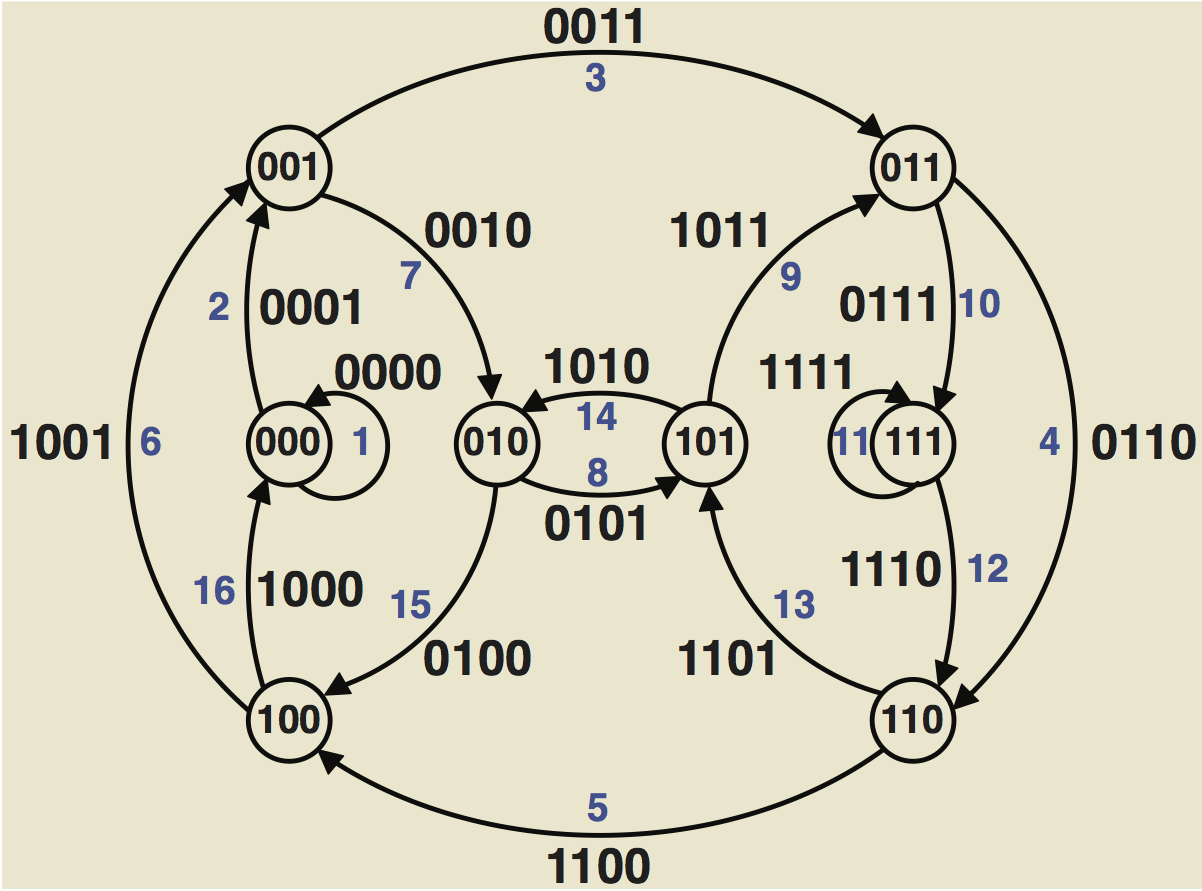
\includegraphics[scale=0.4]{debruijn.png}
  \end{center}
  \caption{deBruijn çizgesi.}
  \label{fig:debruijn}
\end{figure}

de Bruijn çizgelerinin en önemli özelliği Euler döngüsü içeriyor olmalarıdır. Bunun sebebi çok basittir: her köşeye $n$ tane giren kenar ve her köşeden $n$ tane çıkan kenar vardır. Ayrıca, bu çizgenin üzerindeki Euler döngüsü çizgedeki bütün kenarları içerdiği için, bu Euler döngüsü sayesinde ortaya çıkan dizi de $k$ uzunluğundaki olabilecek bütün nk farklı diziyi de içermektedir. Dolayısıyla, Euler döngüsü en baştaki probleme çözüm üretmiş olur.

	Bu noktada karşılaştığımız soru, yukarıda anlatılan de Bruijn çizgesini genom birleştirme problemine nasıl uygulayabileceğimiz olacaktır. Gözlemlenmesi gereken ilk nokta genom birleştirme problemindeki alfabenin 4 harften oluşmasıdır: $\{A, T, G, C\}$. $k$ sayısı ise 50 ve 75 aralığında sabit bir sayı olarak seçilir (100 baz çiftlik diziler için). Seçilen $k$ sayısı kullanılarak her kısa dizinin $k-1$ uzunluğundaki bütün altdizileri ($(k-1)$-mers) bir araya getirilir. Bu $(k-1)$-mer'ler, oluşturulan de Bruijn çizgesindeki köşelere denk gelmektedirler. Kısa dizilerde art-arda gelen ve $k-2$ harfi örtüşen herhangi iki $(k-1)$-mer için de Bruijn çizgesine birer kenar eklenir. Bu eklenen kenar ait olduğu iki $(k-1)$-mer'den oluşan $k$ uzunluğundaki diziye tekabül etmektedir.
	Kısa dizilerinin çok fazla sayıda olması ve $k$ sayısının küçük olması, oluşturulan de Bruijn çizgesinin olası tüm $4^k-1$ tane köşeyi ve $n^k$ tane kenarı içerdiğini varsayabiliriz. Dolayısıyla, oluşturulan de Bruijn çizgesi Euler döngüsü içermektedir ve bu döngünün oluşturduğu uzun dizi tüm kısa dizileri içerdiği için bizim aradığımız hedef genom dizisine denk gelir.
	Elimizdeki milyarlarca kısa diziden oluşturulan de Bruijn çizgesi genomdaki dizi tekrarlanması problemini çözemez. Bunun en başlıca sebebi kısa dizilerin hedef genomu eşit dağılmadan kapsamasıdır. Dolayısıyla, oluşturulan çizgenin kenar ağırlıklarının yüksek olduğu kısımlar aslında birden fazla tekrarlana diziye mi yoksa tekrarlanmayan ama dizileme sırasında çok fazla kapsanan diziye mi tekabül ettiğini ayırt etmek zor bir problemdir. Şekil~\ref{fig:debruijn-repeat} tekrarlanan dizilerin çizge üzerindeki etkilerini göstermektedir:

\begin{figure}[htb]
  \begin{center}
    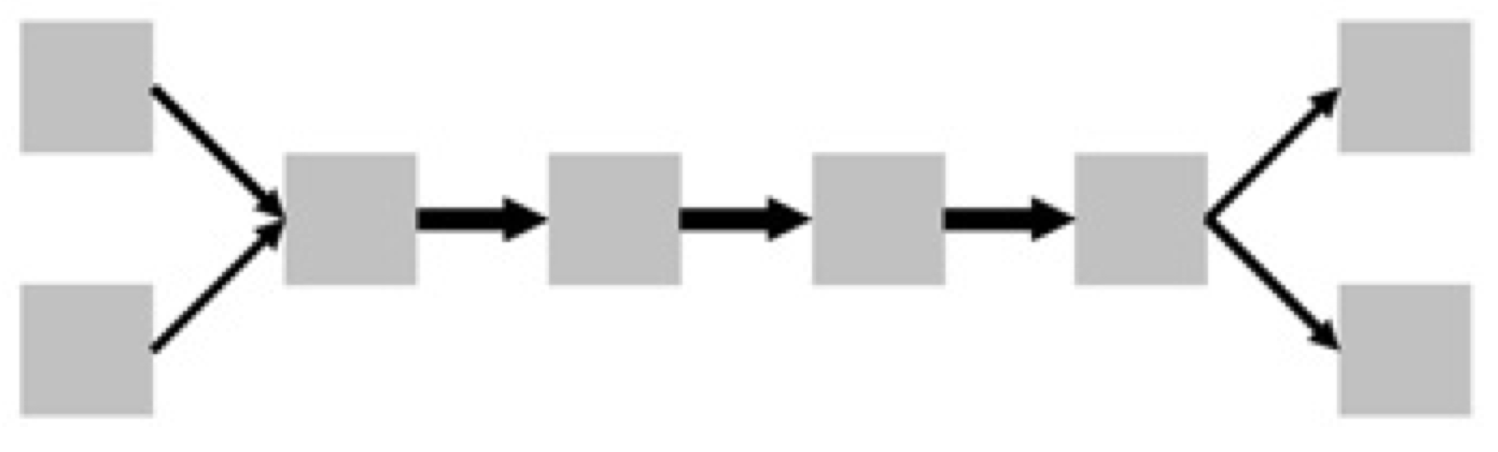
\includegraphics[scale=0.4]{debruijn-repeat-problem.png}
  \end{center}
  \caption{Tekrarlanan dizilerin deBruijn çizgesi üzerindeki etkileri.}
  \label{fig:debruijn-repeat}
\end{figure}

	Şekil~\ref{fig:debruijn-repeat}'de görüldüğü gibi kısa dizilerin uzunluklar tekrarlanan dizilerin uzunluklarından daha kısa (şekildeki köşeler kısa dizilere denk gelmektedir) olduğunda bu tür sorunlar oluşuyor. Ortadaki kalın kenarlar Euler döngüsünde 2 farklı yerde kullanılması gerekirken tek yerde kullanılacaktır. Bu sorunu çözmek için dizileme hata payı yüksek olmasına rağmen ürettiği kısa dizilerin uzunlukları çok uzun olan bir başka dizileme teknolojisinin ürettiği verileri de kullanarak hiperçizge (hypergraph) yapısı altında  yeni bir genom birleştirme algoritması öneriyoruz. Önerdiğimiz yöntemin detaylarına inmeden önce hiperçizge yapısını tanımlayalım:
	
	Hiperçizge $H = (V, X)$ çiftinden oluşmaktadır. $V$ köşelerin kümesini tanımlar, $X = \{E_1, E_2, \ldots, E_n\}$ ise hiperkenarları tanımlar. Burada, $X$ kümesi $V$'nin altkümelerinden oluşur ve $|E_i| \geq 2$ kuralını sağlar. Genel olarak, hiperçizgelerin normal çizgelerden en önemli farkı, hiperkenarların sadece iki köşeyi değil, ikiden fazla köşeyi de birleştirebiliyor olmasıdır.

	Günümüz Yeni Nesil Dizileme cihazlarından iki tanesini ele alalım:

\begin{itemize}
\item Illumina: Dizileme sonucunda ürettiği kısa dizilerin uzunluğu 100-150 baz çiftidir. Uzunluk çok kısa olmasına rağmen, bu teknolojinin hata payı 0.01\% civarındadır.
\item Pacific Biosciences (PacBio): Dizileme sonucunda ürettiği kısa dizilerin ortalama uzunluğu 8000 baz çifti civarındadır. Ancak diziler uzun olmalarına rağmen, bu teknolojinin hata payı 10\%-15\% civarındadır.
\end{itemize}

	Illumina'nın çıktılarının hata payı çok düşük olduğu için, bu teknoloji çok yaygın kullanılmaktadır. Ancak kısa dizilerin uzunluğu 100 baz çifti olduğu için, hedef genomdaki uzunluğu 100'den daha uzun olan tekrarlanan dizilerin belirlenmesi çok zordur. Bizim önerdiğimiz çözüm 2 aşamalıdır:

\begin{enumerate}
\item Geleneksel de Bruijn çizgesi yöntemini ve sadece Illuminadan gelen verileri kullanarak de Bruijn çizgesinin oluşturulması.
\item PacBio cihazından gelen her bir kısa dizi için 1. aşamada oluşturulan çizgeye 1 tane hiperkenarın eklenmesi. Bu eklenen hiperkenar, ait olduğu kısa dizinin içerdiği tüm $(k-1)$-merleri birleştirir. 
\end{enumerate}

İki aşama sonucunda elde edilen hiperçizge Şekil~\ref{fig:hypergraph}'de gösterilmiştir.

\begin{figure}[htb]
  \begin{center}
    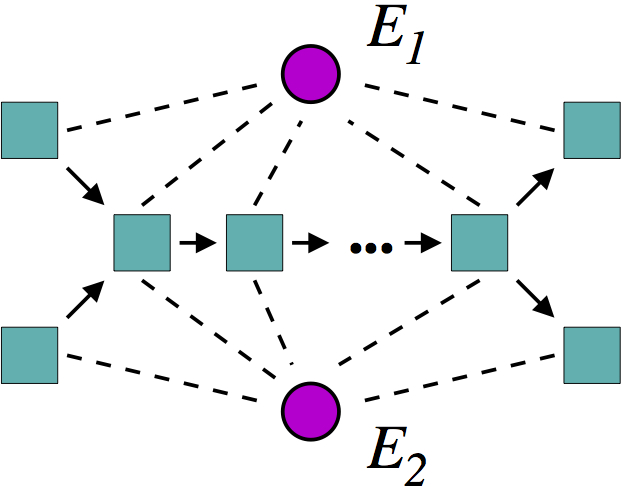
\includegraphics[scale=0.4]{hypergraph.png}
  \end{center}
  \caption{Hiperçizge.}
  \label{fig:hypergraph}
\end{figure}



	Bu modellemenin avantajları aşağıda listelenmiştir:
PacBio'dan gelen kısa dizilerin uzunlukları kadar uzun tekrarlanmalar çözümlenebilir.
PacBio'nun dizileme hata payı çok yüksek olmasına rağmen, elde edilen nihai genom Illumina verisinden elde edilen verinin hata payına göre oluşturulur.
Bu model sadece bu iki veri kaynağı için değil, başka veri kaynaklarından gelen veriler için de kullanılabilir; örneğin Roche/454, Ion Torrent, Oxford Nanosciences, Moleculo, vb.
